\section{Methods}




\begin{figure}[htbp]
  \centering
  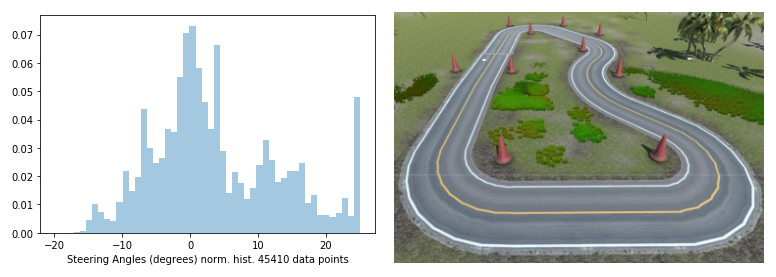
\includegraphics[width=\textwidth]{Figures/GeneratedTrackPlusHistogram.png}
 \caption{
 Normalized histogram of Unity 3D SDSandbox steering angles for 45410 image frames. The corresponding track (small\_looping\_couse) is shown on the right
 }
 \label{fig:GeneratedTrackPlusHist}
\end{figure}

\begin{figure}[htbp]
 \centering 
 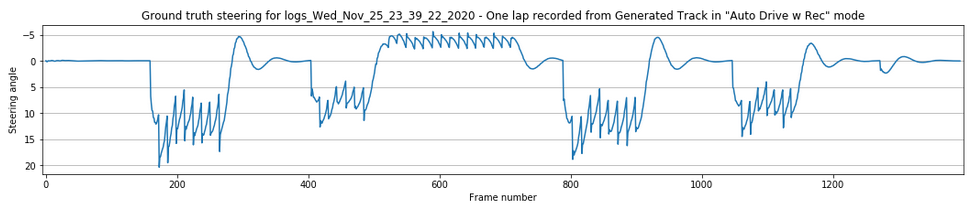
\includegraphics[width=\textwidth]{Figures/genTrackOneLap_logs_Wed_Nov_25_23_39_22_2020_ground_truth_steering_angles.png}
 \caption{Ground truth steering values for logs\_ Wed\_ Nov\_ 25\_ 23\_ 39\_ 22\_ 2020 recorded log.}
 \label{fig:genTrackOneLap_logs_Wed_Nov_25_23_39_22_2020_ground_truth_steering_angles} 
\end{figure}

\begin{figure}[htbp]
\centering
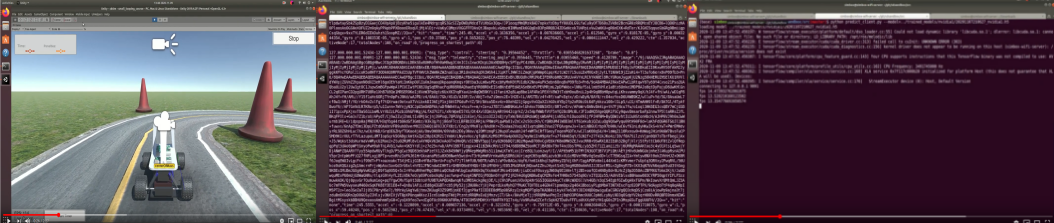
\includegraphics[width=\textwidth]{Figures/SimTCPPred.png}
\caption{Stills of video \url{https://youtu.be/9z0mMtOnUUc} showing left to right: SDSandbox simulated car going around the Generated Track course, TCP Debug (tcpflow) and prediction engine (predict\_ client.py) running}
\label{fig:SimTCPPred}
\end{figure}

\begin{figure}[htbp]
 \centering 
 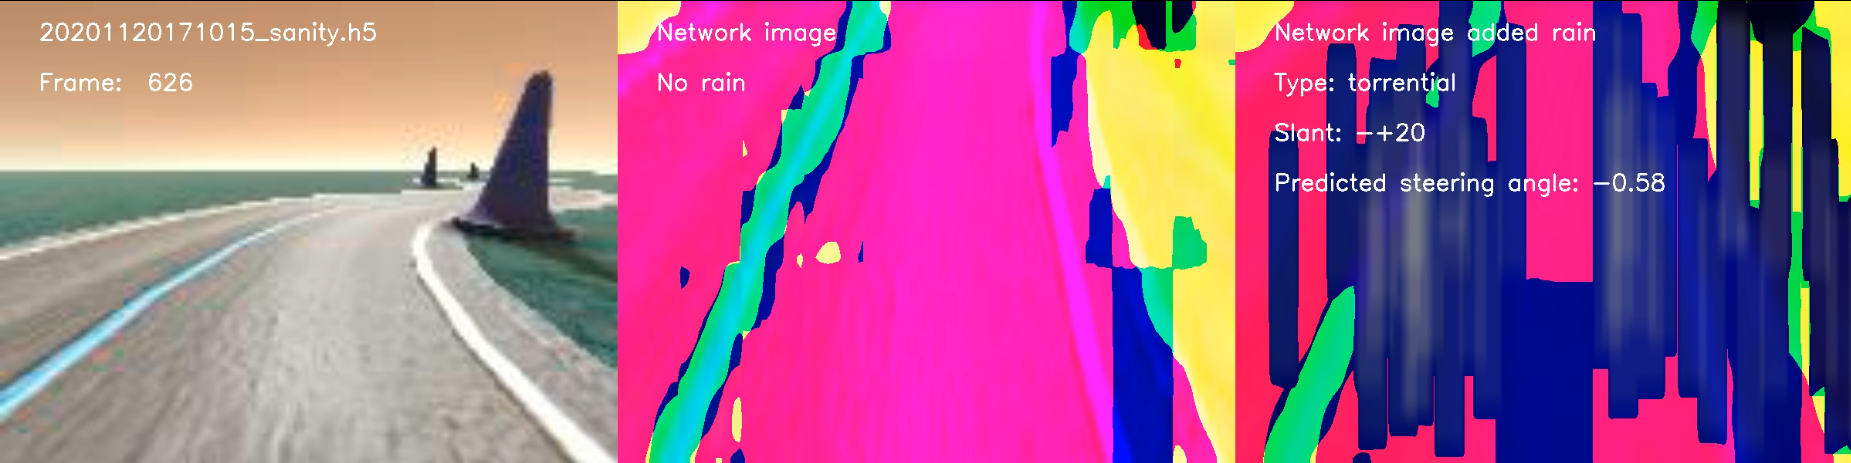
\includegraphics[width=\textwidth]{Figures/tcpflow_Run43.png}
 \caption{Video still showing left to right, the acquired image supplied by the simulator, a processed network image with no rain and the same image with torrential rain added. This last being the image presented to the network. A video was recorded in run \ref{app_res:43}, \url{https://youtu.be/57jwwcjbfdE}, showing the model driving off the track.}
 \label{fig:tcpflow_Run43} 
\end{figure}

%%%%%%%%%%%%%%%%%%%%%%%%%%%%%%%%%%%%%%%%%%%%%%%%%%
% Generated Road, sim on left and detail on right
%%%%%%%%%%%%%%%%%%%%%%%%%%%%%%%%%%%%%%%%%%%%%%%%%%

\begin{figure}[htbp]
 \centering 
 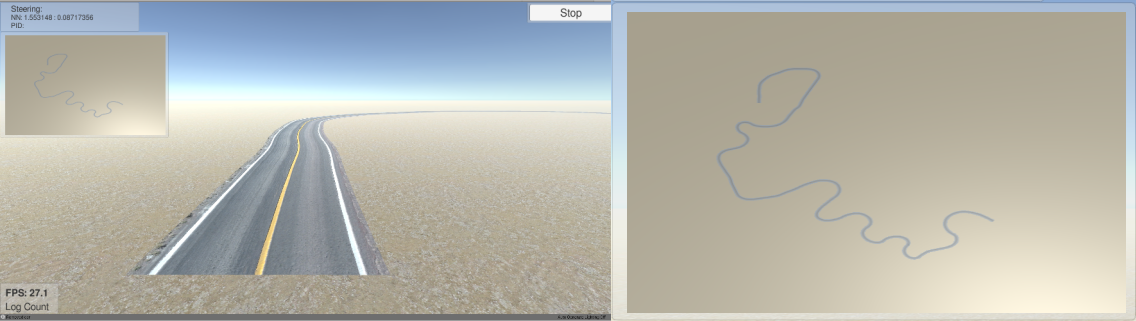
\includegraphics[width=\textwidth]{Figures/run-93-94-generated-road.png}
 \caption{The randomly generated Generated Road circuit used in runs 93 and 94. Left image is a view of the simulator as presented on computer desktop, the right image is the augmented detail showing the Generated Road circuit, the same inset on left image.}
 \label{fig:run-93-94-generated-road-res} 
\end{figure}

We created a simulation and got the network to predict the outcome.

The evaluation can be performed qualitatively using a simulator as described in (TODO MISSING REF) to observe the simulated vehicle self-driving with respect to oversteering and understeering, crashes providing pass/fail metric.

The proposed quantitive evaluation metric is \textit{goodness-of-steer}. In equation     \ref{eq:goodness_of_steer}:

\begin{equation}
    \label{eq:goodness_of_steer}
    g_s(p,g) = \frac{\sum_i^N \lvert p(i)-g(i) \rvert }{N} \times n_c
\end{equation}
where $p,g$ are prediction and ground truth arrays,  $N$ is the number of predictions and $n_c$ is the normalization constant (25 in example shown, 1 for values not normalized), which in this case is the maximum steering angle for the SDSandbox simulated vehicle. In plain english, $g_s$ is defined as the sum of the absolute value of the difference between prediction and ground truth values, divided by the number of predictions multiplied by a normalization constant, that is the steering error average over all predictions. 